% !TEX encoding = UTF-8
% !TEX TS-program = pdflatex
% !TEX root = ../tesi.tex
% !TEX spellcheck = it-IT

%**************************************************************
\chapter{Introduzione}
\label{cap:introduzione}
%**************************************************************
xxxx
Introduzione al contesto applicativo.\\

\noindent Esempio di utilizzo di un termine nel glossario \\
\gls{api}. \\

\noindent Esempio di citazione in linea \\
\cite{site:agile-manifesto}. \\

\noindent Esempio di citazione nel pie' di pagina \\
citazione\footcite{womak:lean-thinking} \\

%**************************************************************
\section{L'azienda}

VIC è stata fondata da Alessio Bisutti che, dopo aver sviluppato una lunga esperienza nel campo ispettivo, ha deciso di costituire una società in grado di offrire ai propri clienti un servizio professionale, chiaro ed affidabile, appoggiandosi sulle nuove tecnologie.\\
VIC iniziò a Venezia 7 anni fa come piccola società di ispezione locale ed ora il gruppo VIC è uno dei più grandi attori del mercato globale.\\
Fin dall'inizio, l'obiettivo principale di VIC è stata la riduzione del tempo tra ispezione e reporting al cliente. Ora l'obiettivo è raggiunto, perché VIC sta fornendo ai suoi clienti tutti i risultati e le informazioni importanti in tempo reale, senza alcun ritardo, grazie agli investimenti fatti nel campo della tecnologia e delle applicazioni mobile.\\
VIC è la prima ed unica azienda in campo ispettivo ad offrire un'ampia gamma di servizi tecnologici a completa disposizione dei propri clienti. 

%**************************************************************
\section{L'idea}

Mansioni come determinare la corretta forma, peso, quantità e dimensioni degli oggetti da ispezionare sono tra le più importanti per i controlli effettuati dall'azienda.\\
Gli ispettori possono scattare molte fotografie, prendere appunti e sfruttare la loro esperienza per fornire stime accurate; si è manifestata però la necessità di affiancare queste ultime a dei dati quanto più possibile oggettivi e rapidi da ottenere.\\
Da qui nasce l'idea di fornire agli ispettori uno strumento informatico in grado di effettuare queste stime. Grazie alla ricostruzione computerizzata resa disponibile dai \emph{Tango device} sarà possibile non solo visualizzare su uno schermo il modello 3D del soggetto della ispezione, ma anche ottenere ulteriori vantaggi come:
\begin{itemize}
	\item Avere una stima del volume e quindi del peso della materia prima.
	\item Confrontare l'oggetto con un modello idea, permettendo così un rapido controllo eventuali di danni o deformazioni.
\end{itemize}

\section{Il Prodotto}
L'applicazione prodotta risponde, in maniera minimale, alle esigenze citate nel punto precedente.\\
La sua realizzazione presenta molti punti critici e rischi piuttosto difficili da prevedere. Per questo sono stati realizzati molti prototipi, al fine di escludere vie non percorribili e trovare una soluzione soddisfacente.\\
Lo scopo principale della applicazione lato tablet è quello di rilevare ed elaborare un corretto \emph{Point Cloud} dell'oggetto che si vuole ispezionare.\\
Un \emph{Point Cloud} non è altro che una descrizione algebrica di un oggetto tridimensionale ottenuta tramite un insieme, il più possibile fitto, di punti che lo compongono. I dispositivi Tango infatti, grazie al sensore di profondità, cercano di rilevare le triplette di coordinate del maggior numero di punti possibile. Sfruttando questi dati è possibile posizionare dei punti nello spazio in maniera da fornire all'utente una rappresentazione comprensibile dell'oggetto.
\begin{figure}[!h] 
    \centering 
    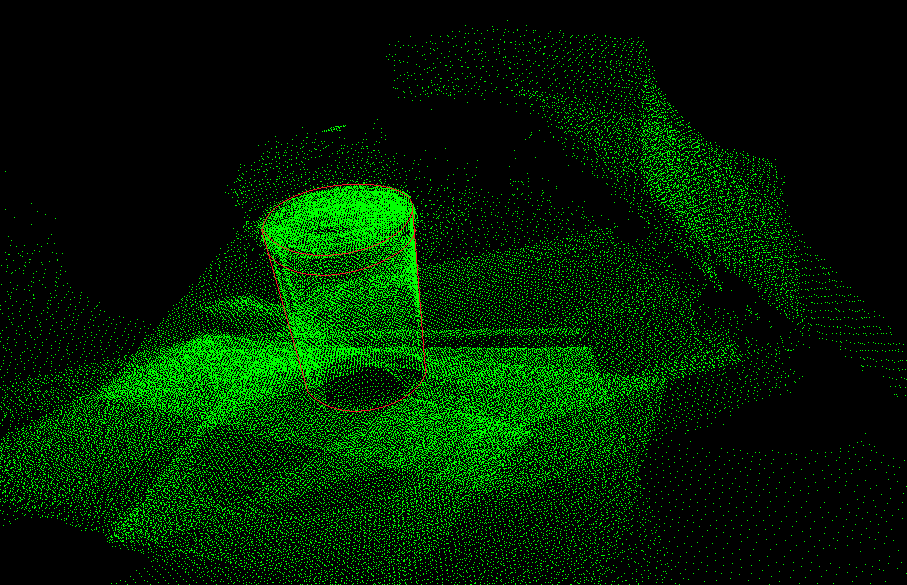
\includegraphics[width=0.9\columnwidth]{pointClouds/bidoneConico.png} 
    \caption{Point Cloud di un bidone Conico}
\end{figure}

\subsection{Primo prototipo}
Il primo protitpo realizzato risponde all'esigenza di catturare e salvare in formato leggibile da un \emph{render} grafico i dati forniti dal sensore di profondità.
Nella sua semplicità ha dato modo allo studente di testare la stabilità delle \emph{API} e produrre della documentazione interna che riportava quali fossero i metodi delle \emph{API} da utlizzare e quali fossero invece quelli poco stabili, sperimentale o addirittura non ancora implementati dal produttore.

\subsection{Secondo prototipo: Cloude}
Un solo \emph{Point Cloud} non è sufficiente a ricostruire un oggetto. Ovviamente il dispositivo, registrando la nuvola di punti inquadrata in un determinato istante, riesce a rilevare solamente i punti che "riesce a vedere": i punti presenti nella parte posteriore dell'oggetto scansionato non possono essere "visti" e conseguentemente nemmeno misurati.\\
Se si vuole avere una ricostruzione completa e non solamente di una facciata è necessario prendere più rilevazioni ed unirle assieme.\\
Questo prototipo, denominato \emph{Cloude}, è stato realizzato allo scopo di rispondere a questa esigenza. L'idea che ne sta a fondamento è la seguente:
\begin{itemize}
	\item Permettere all'utente di scattare alcune foto all'oggetto, quindi di rilevare diversi \emph{Point Cloud}.
	\item 
	\item Una volta acquisito i dati dal Point Cloud usare la posizione e la rotazione del dispositivo per trasformare punto per punto la nuvola rispetto a delle coordinate assolute.
\end{itemize}

%**************************************************************
\section{Organizzazione del testo}
xxxx
\begin{description}

    \item[{\hyperref[cap:processi-metodologie]{Il secondo capitolo}}] descrive ...
    
    \item[{\hyperref[cap:descrizione-stage]{Il terzo capitolo}}] approfondisce ...
    
    \item[{\hyperref[cap:analisi-requisiti]{Il quarto capitolo}}] approfondisce ...
    
    \item[{\hyperref[cap:progettazione-codifica]{Il quinto capitolo}}] approfondisce ...
    
    \item[{\hyperref[cap:verifica-validazione]{Il sesto capitolo}}] approfondisce ...
    
    \item[{\hyperref[cap:conclusioni]{Nel settimo capitolo}}] descrive ...
\end{description}

Riguardo la stesura del testo, relativamente al documento sono state adottate le seguenti convenzioni tipografiche:
\begin{itemize}
	\item gli acronimi, le abbreviazioni e i termini ambigui o di uso non comune menzionati vengono definiti nel glossario, situato alla fine del presente documento;
	\item per la prima occorrenza dei termini riportati nel glossario viene utilizzata la seguente nomenclatura: \emph{parola}\glsfirstoccur;
	\item i termini in lingua straniera o facenti parti del gergo tecnico sono evidenziati con il carattere \emph{corsivo}.
\end{itemize}